\section{From bulk comparisons to quenched curves}
\label{sec:curves}

We now work at the physical critical point identified in
Theorem~\ref{crit:physical}.  The bulk comparisons of
Section~\ref{sec:crossings} will yield couplings between the target
interface and pure interfaces in slightly displaced domains.  The pure
marginal in each coupling will remain fixed after conditioning on the
environment.  This conditional marginal property is what turns the
geometric argument into convergence of quenched probability measures.
In this section, unsubscripted probabilities and expectations include
the sampled spins and coupling randomness as well as the environment.

Fix the marked Jordan domain and an admissible approximation from
Theorem~\ref{thm:main}, and write
\[
 D_n=\delta_nD_{V_n},\qquad
 \Gamma_n=\delta_n\gamma(P).
\]
The contour--spin correspondence gives a nearest-neighbor ferromagnetic
spin law with the actual exterior pins induced by the fixed completion
$P_{o,n}$.  Every bond meeting $V_n$, including a bond crossing its boundary,
retains its prescribed coupling.  The correspondence is the bijection
proved in Lemma~\ref{intro:contour-spin}.  Thus the conditional law of $\Gamma_n$ given the original
environment $\omega$ is exactly $Q_{n,\omega}$.

Along a subsequence the designation of the two signed boundary arcs is
fixed.  Denote the open plus and minus arcs of $\partial D$ by $I_+$ and
$I_-$.  All paths and crossings below use the fixed triangulation and
resolution convention of Section~\ref{sec:crossings}.  Changing between
its interpolated contour and the prescribed locally resolved curve
changes $d_{\mathrm{curv}}$ by $O(\delta_n)$: match occupied edges in their
traversal order, and match the connections inside the vertex disks.

\subsection{A conditional comparison device}

We first isolate the probability argument used to transfer a finite
family of boundary barriers.  For vectors in $\{0,1\}^m$, the symbol
$\preceq$ denotes coordinatewise order, and for their laws it denotes
the existence of a coupling supported on that order.

\begin{lemma}[Conditioning and gluing at fixed environment]
\label{curv:conditional-gluing}
Let $\lambda$ be a deterministic law on a finite set, let $\mu_\omega$
be an environment-dependent law on another finite set, and let
$U$ and $W$ be maps from these sets to $\{0,1\}^m$.
Let $p$ and $q_\omega$ be laws of $(e,v)\in\{0,1\}\times\{0,1\}^m$,
where $p$ is deterministic and $p(e=1)\ge a>0$.  Suppose that
\[
 \mathcal L_\lambda(U)\preceq p(v\in\cdot\mid e=1),\qquad
 q_\omega(v\in\cdot\mid e=1)\preceq\mathcal L_{\mu_\omega}(W)
\]
whenever $q_\omega(e=1)>0$.  Put
$\varepsilon(\omega)=\|p-q_\omega\|_{\TV}$.  There is a measurable
family of couplings $\pi_\omega$ of $\lambda$ and $\mu_\omega$ such that
\begin{equation}
 \E_{\mathrm{env}}\,
 \pi_\omega\{U\npreceq W\}
 \le \frac{6}{a}\E_{\mathrm{env}}\varepsilon(\omega).
 \label{curv:gluing-error}
\end{equation}
In particular, the first marginal under $\pi_\omega$ is $\lambda$ for
every environment, including those on which the comparison fails.
\end{lemma}

\begin{proof}
On $\{\varepsilon\le a/2\}$, the second conditioning probability is at
least $a/2$.  Subtracting the two conditional probability fractions gives
\[
 \bigl\|p(v\in\cdot\mid e=1)
       -q_\omega(v\in\cdot\mid e=1)\bigr\|_{\TV}
 \le \frac{4\varepsilon(\omega)}a.
\]
Couple these two vectors maximally and glue this coupling to the two
order couplings.  Extend the outer vectors to samples with laws
$\lambda$ and $\mu_\omega$ by their conditional laws given $U$ and $W$.
The outer vectors are ordered unless the two middle vectors disagree.
On $\{\varepsilon>a/2\}$ take any coupling with the same outer
marginals.  Markov's inequality bounds this exceptional environmental
probability by $2\E_{\mathrm{env}}\varepsilon/a$, proving
\eqref{curv:gluing-error}.  All sets are finite.  The coupling matrices
and subsequent conditional probabilities can be selected measurably;
for instance, fix an enumeration of feasible basic solutions of the
finite coupling constraints and choose the first available one.
\end{proof}

The lemma compares conditional laws for each fixed environment.  It
does not condition the environment on $e=1$; doing so would change the
environmental distribution and lose the marginal property needed at
the end of the proof.

\subsection{Displaced domains and finite boundary barriers}

We record the precise geometric constructions from the companion that
will be used.  They are deterministic statements about Jordan domains,
signed paths, and the prescribed triangulation.

Fix a Schoenflies homeomorphism $\Psi$ of the plane taking the unit disk
to $D$, the points $1,-1$ to $a,b$, and the upper semicircle to $I_+$.
For each sufficiently small displacement $h>0$, there are polygonal
marked Jordan domains $A_h^-$ and $A_h^+$, with marks
$a_h^\pm,b_h^\pm$ tending to $a,b$,
whose boundary parametrizations tend uniformly to that of $D$ as
$h\downarrow0$.  The superscript indicates the favored spin sign.  For
$A_h^-$, its middle plus arc is displaced outside $D$, and the rest of
its boundary is displaced inside $D$, with transitions near the marks.
There are two disjoint polygonal cutting corridors $C_h^-$ and $C_h^+$,
with slightly larger disjoint reveal regions, having the following
properties:
\begin{enumerate}
 \item The minus corridor and its reveal region lie outside
 $\overline{A_h^-}$.  A lengthwise minus crossing separates the minus
 boundary of $D_n$ from the common central region.
 \item The plus corridor and its reveal region lie outside
 $\overline D$.  A lengthwise plus crossing separates the plus boundary
 of $A_h^-$ from that region.
 \item The corridor caps extend across the boundary portions they cut.
 All the stated separations have positive clearance at fixed $h$ and
 persist for all sufficiently large $n$.
\end{enumerate}
An \emph{allowed plus strip} is a polygonal topological rectangle whose
closure lies in $A_h^-$ on the central side of the cuts, disjoint from the reveal
regions, whose two end gates lie outside $\overline D$ on its enlarged
plus side.  Every contact of the strip with $\partial D$ is on $I_+$,
away from $a,b$, and the strip lies in
$\Psi(\{\rho<1+h/2\})$, with fixed positive clearance from that
outer bound.  A crossing in the target is defined after filling the
portions outside $D_n$ virtually with plus.  For $A_h^+$ the construction
is obtained by interchanging plus and minus.  These objects, including
the requirements on strip gates, are constructed in
\cite[Section~7, ``Fixed displaced domains and their boundary
incidences'']{S}.

Figure~\ref{curv:boundary-squeeze} shows the distinction between the
corridor caps and the strip gates.  The plus corridor crosses the minus
shoulders of $A_h^-$, whereas the strip gates lie inside its enlarged
plus portion.  These placements give the ordered incidences used below.

\begin{figure}[tbp]
 \centering
 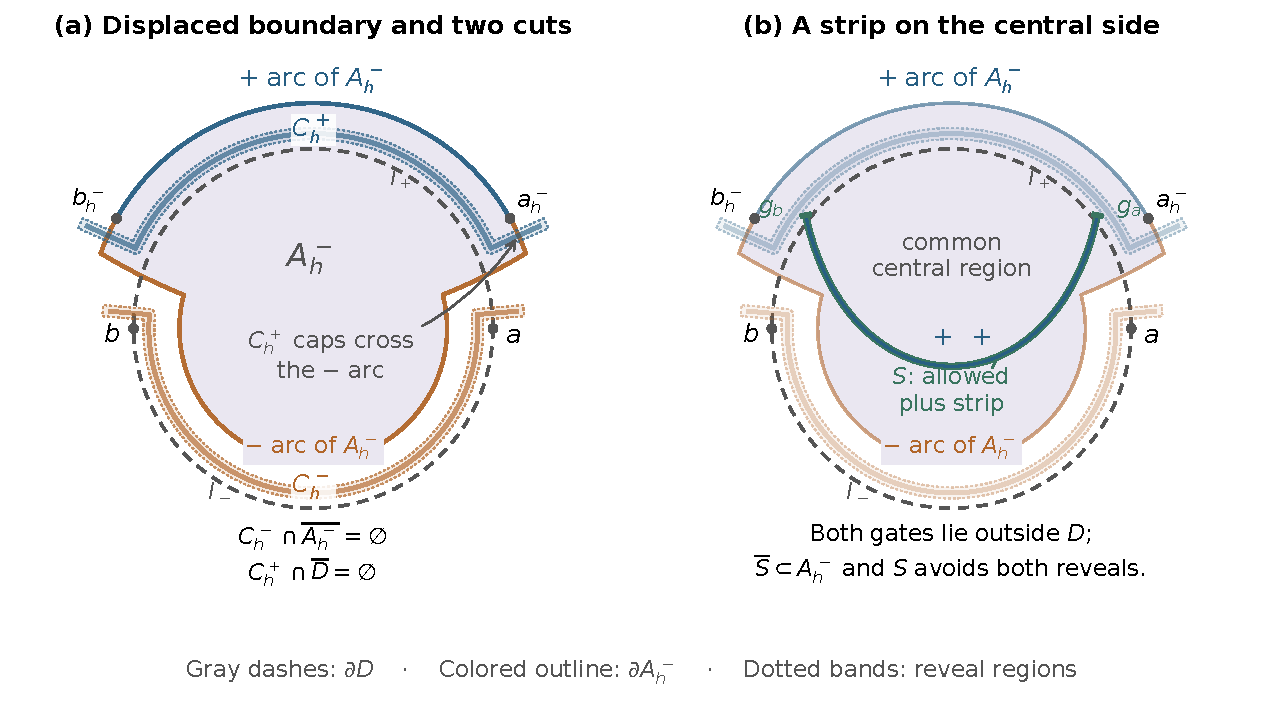
\includegraphics[width=\textwidth]{figures/boundary-squeeze.pdf}
 \caption{Boundary squeeze favoring minus, in fixed Schoenflies
 coordinates.  (a) The dashed circle is $\partial D$; the shaded
 comparison domain has blue plus and orange minus boundary arcs.
 The blue corridor $C_h^+$ lies outside $D$, with caps crossing the
 minus shoulders of $\partial A_h^-$; the orange corridor $C_h^-$ lies
 outside $A_h^-$ and screens the minus arc of $D$.  Dotted bands are
 disjoint reveal regions.  (b) An allowed plus strip $S$ lies on the
 central side of both cuts.  Its gates $g_a,g_b$ are outside $D$, while
 its closure remains inside $A_h^-$ and avoids the reveal regions.
 The thin blue line inside $S$ illustrates a plus spin crossing.
 The drawing shows the preliminary topological configuration; the
 proof uses close polygonal approximations in the physical plane.
 Displacements and widths are schematic.}
 \label{curv:boundary-squeeze}
\end{figure}

The boundary hypothesis in Theorem~\ref{thm:main} is exactly what is
needed here.  If $c$ parametrizes $\partial D$, then $\phi_n\circ c$
converges uniformly to $c$.  Winding numbers therefore determine the
same inside and outside on each compact set disjoint from $\partial D$,
and the marked boundary order gives the same signed-arc incidences away
from the marks.  Fine teeth of $D_n$ remain in a shrinking boundary
collar and cannot enter any of the fixed clearances above.  Virtual
filling records a geometric crossing only: it changes neither a
coupling nor an exterior pin.  The corner check in
\cite[Section~7, paragraph following ``Fixed-geometry boundary
squeeze'']{S} ensures that such a signed path cannot cross the target
resolved contour, including at reflex corners.

\begin{proposition}[Quenched transfer of a finite strip family]
\label{curv:strip-transfer}
Fix $h>0$ and a finite family of allowed plus strips in $A_h^-$.  Let
$\Sigma_{h,n}^-$ have the pure Dobrushin spin law in an ordinary lattice
approximation of $A_h^-$, and let $\Sigma_{n,\omega}$ have the target
spin law.  These samples admit couplings conditional on $\omega$ whose
two marginals are the stated laws and for which
\begin{equation}
 \Prob\!\left(
   \text{every strip crossed by plus in }\Sigma_{h,n}^-
   \text{ is crossed by plus in }\Sigma_{n,\omega}
             \right)=1-o(1).
 \label{curv:strip-order}
\end{equation}
The probability in \eqref{curv:strip-order} includes environment and
coupling randomness.  The pure marginal conditional on $\omega$ is
its deterministic Dobrushin law.  The corresponding assertion holds
for minus strips in $A_h^+$.
\end{proposition}

\begin{proof}
Put the corridors, their reveal regions, and the finitely many strips
inside a torus chart with a fixed positive external buffer.  Choose a
torus period allowed by Proposition~\ref{cross:torus-comparison}.  In
this chart use the same bond environment as the target; complete the
torus with independent bonds.  Write $E_h$ for the event that both
cutting corridors have their prescribed lengthwise colored crossings,
and write $V$ for the vector of ordinary plus crossings of the strips
on the torus.  The pure buffered crossing bounds give
\[
 p_n(E_h)\ge a_h>0,
 \qquad
 p_n=\mathcal L_0(\1_{E_h},V),
\]
for all sufficiently fine meshes.  Here $a_h$ may depend on the fixed
geometry.  With $q_{n,\omega}$ denoting the corresponding quenched
torus vector law, Proposition~\ref{cross:torus-comparison} gives
\begin{equation}
 \E_{\mathrm{env}}\|q_{n,\omega}-p_n\|_{\TV}\longrightarrow0.
 \label{curv:middle-tv}
\end{equation}
At this stage the environmental expectation includes the independently
added torus bonds.

We verify the two order comparisons needed for
Lemma~\ref{curv:conditional-gluing}.  In either torus, conditional on
$E_h$, reveal the prescribed crossing nearest the exterior side of each
corridor.  The stopped reveal of
\cite[Section~6, Lemma ``Reveals with a monochromatic facing boundary'';
Section~7, proof of
``Fixed-geometry boundary squeeze'']{S} leaves only pins of the
prescribed color facing the unrevealed center.  The transcript already
determines crossing existence, so no additional conditioning on $E_h$
remains in that center.  Disjoint reveal regions allow both explorations.

First compare the pure Dobrushin law in $A_h^-$ with the conditioned
pure torus.  The revealed plus path is an upper plus pin against a
lower free spin.  It screens the plus arc of $A_h^-$; every accessible
remaining boundary incidence is a lower minus pin against an upper free
spin.  Meetings of a cut and boundary give upper plus against lower
minus.  The minus reveal is outside $A_h^-$.  Ferromagnetic boundary
comparison therefore puts the pure-domain strip vector below
$p_n(V\in\cdot\mid E_h)$.

Next compare the conditioned random torus, as the lower law, with the
target, as the upper law.  They have identical couplings on every bond
in their common free region.  The minus path screens the target minus
arc.  The remaining boundary incidences, with upper entry first, are
exactly
\[
 (+,\mathrm{free}),\qquad(\mathrm{free},-),\qquad(+,-).
\]
Each comparison follows by conditioning a free spin to its extremal
value and using the nearest-neighbor ferromagnetic order.  This also
explains why no comparison between different random bond strengths is
needed.  The source's geometric incidence check, including the
corridor caps, shows that these are all incidences encountered by the
common components containing the strips.  A nearest-neighbor edge
cannot cross the interior of a separating triangulated diagonal.
Virtual plus values outside $D_n$ give the same order for portions of
a strip that exit and reenter the target.  Thus
$q_{n,\omega}(V\in\cdot\mid E_h)$ is below the target strip vector.

Apply Lemma~\ref{curv:conditional-gluing} with $a=a_h$ and
\eqref{curv:middle-tv}.  It gives \eqref{curv:strip-order}, extending
the strip vectors to the complete spin samples with their conditional
laws.  Finally average over the extra torus bonds while retaining the
original environment.  The conditional pure marginal is unchanged,
and the target marginal never used the extra bonds.  Interchanging
the signs proves the other assertion.
\end{proof}

\subsection{The geometric curve inputs}

For completeness, we state the three further conclusions of the
companion's boundary argument in the form needed here.  Their geometric
parts apply to marked target interfaces with the designated boundary
signs and noncrossing signed barriers; they assume no symmetry of the
target spin law.

\begin{lemma}[Finite strips and limiting barriers]
\label{curv:geometric-input}
For either sign of displacement, the continuum laws
$\mathrm{SLE}_3(A_h^\pm;a_h^\pm,b_h^\pm)$
converge in $d_{\mathrm{curv}}$, as $h\downarrow0$, to
$\mathrm{SLE}_3(D;a,b)$.  Given errors $\eta_j\downarrow0$, one can
choose displacements $h_j\downarrow0$ and, for each $j$, a finite
deterministic family of allowed strips of each sign with the following
property.  Outside an event of pure probability at most $\eta_j$, a
continuum comparison chord selects a strip from its family and traverses
it with strict margins from its long sides and across its end gates.
Only terminal pieces of diameter at most $\eta_j$ are omitted.  The
strip has cross-sections of diameter at most $\eta_j$ following a simple
prototype within $\eta_j$, in $d_{\mathrm{curv}}$, of that middle subarc.
For all sufficiently fine pure lattice approximations, the pure lattice
interface selects such a strip and has the corresponding traversal,
with geometric errors at most $2\eta_j$; its adjacent signed spin path
crosses the strip, outside an event of probability at most $2\eta_j$.

Suppose the prescribed target contours in $D_n$, with their designated
boundary signs, have the corresponding two signed strip barriers with
failure probability tending to zero along such a sequence, and let
$(K,L,U)$ be any joint subsequential limit of their traces and the two
comparison chords, in Hausdorff distance for the traces and
$d_{\mathrm{curv}}$ for the comparison chords.  Here $L$ is the limit
from $A_h^-$ and $U$ the limit from $A_h^+$.  Then almost surely
\begin{equation}
 K\subset\overline{M(L)}\cap\overline{P(U)}.
 \label{curv:forbidden-sides}
\end{equation}
For a simple chord $C$ in $D$, $P(C)$ and $M(C)$ denote the components
of $D\setminus C$ adjacent to $I_+$ and $I_-$; closures are taken in
$\overline D$.
\end{lemma}

\begin{proof}[Source and scope]
The first assertions are
\cite[Section~7, ``From fixed strip tests to limiting barriers'']{S}.
Uniform boundary parametrization gives uniform convergence of the
normalized conformal maps on the closed disk, including the two marks.
Mapping one disk $\mathrm{SLE}_3$ by these maps proves the displaced
continuum convergence.  For fixed $h$, only pure convergence in an
ordinary polygonal approximation is used.

The finite family is obtained by covering favorable simple comparison
chords with open neighborhoods described by rational polygonal strips,
transverse gates, and strict crossing margins.  Compact middle subarcs
are in $D$; the two short terminal pieces tend to the marks.  A
countable such cover has a finite subfamily carrying arbitrarily large
probability.  Its entire list is fixed before taking the lattice limit;
the sampled pure chord may select a strip only after the joint vector
coupling has been made.  Following the signed side of the lattice
interface supplies the crossing with $O(\delta_n)$ drawing error.

The last assertion is the winding and boundary-order argument of
\cite[Section~7, ``Forbidden sides, order, and identification of the
trace'']{S}.  A signed crossing in one of these strips blocks a target
contour from the corresponding side.  To include the open signed
boundary arc, erase loops from the crossing and close it outside $D_n$.
In the fixed $\Psi$ coordinates, take radial connectors from its gates
to a circle $\rho=\rho_*>1$ and the circular arc on the signed side,
where $\rho_*$ is independent of $h,n$.  At fixed $h$, the added path
has positive clearance from $\overline D$ and hence lies outside $D_n$
for large $n$.  Include this threshold in the diagonal choice.  The
target marks are on the zero-winding side of the closed barrier.  As
the strip widths and terminal errors vanish, the gate centers tend
to the marks, while the fixed-radius closure stays a positive distance
beyond every compact subarc of the signed boundary.  The winding
exclusions therefore hold on every compact neighborhood of the
forbidden side or boundary arc, giving
\eqref{curv:forbidden-sides}.  The argument uses only the deterministic
geometry and noncrossing of opposite signed paths with the target
contour; it applies to the couplings in
Proposition~\ref{curv:strip-transfer}.
\end{proof}

\begin{lemma}[Ordered chords with equal laws]
\label{curv:ordered-chords}
Let $L,U$ be random simple chords from $a$ to $b$ with their interiors
in $D$, and let $K\subset\overline D$ be random, compact, connected,
and contain $a,b$.  If \eqref{curv:forbidden-sides} holds almost surely,
then $P(L)\subset P(U)$ almost surely.  If $L$ and $U$ have the same
trace law, then $K=L=U$ as compact sets almost surely.
\end{lemma}

\begin{proof}
This is \cite[Section~7, Lemma ``Ordered chords with equal laws'']{S}.
Here is the argument.  A point of $P(L)\cap M(U)$ could be connected
inside this union to both signed boundary arcs.  Removing loops gives
a crosscut between those arcs that avoids $K$.  Its endpoints
alternate with $a,b$, so it separates $a$ from $b$, contradicting the
connectedness of $K$.  Hence $P(L)\subset P(U)\cup U$.  No point of
$U$ can belong to the open set $P(L)$, since every neighborhood of an
interior point of $U$ meets $M(U)$.  Thus $P(L)\subset P(U)$.

Use a fixed Schoenflies homeomorphism to the disk and take the planar
areas of the images of these two plus sides.  They are bounded, ordered
random variables with the same distribution, so their difference
vanishes almost surely.  If the inclusion of plus sides were proper,
take $z\in P(U)\setminus P(L)$.  It either lies in $M(L)$, or lies on $L$.
In the latter case a neighborhood of $z$ inside $P(U)$ meets $M(L)$,
by the two-sidedness of a Jordan chord.  In either case the difference
contains a nonempty open subset of $M(L)$, and hence has positive area.
The plus sides are therefore equal, and so are their interior boundary
chords.  By \eqref{curv:forbidden-sides}, $K$ lies on this chord.  The
inverse chord parametrization maps it to a connected subset of $[0,1]$
containing both endpoints, which is all of $[0,1]$.
\end{proof}

The remaining issue is traversal order: Hausdorff convergence alone
would allow repeated forward and backward travel close to one simple
chord.  The next source lemma isolates the required exclusion.

\begin{lemma}[Progress criterion for the curve metric]
\label{curv:progress}
Let $g_n$ be simple oriented curves with endpoints tending to $a,b$,
and let $G$ be a continuous injective chord with those endpoints and
interior in $D$.  Suppose their traces converge to the trace of $G$.
There are continuous $u_n:[0,1]\to[0,1]$ with endpoint values tending
to $0,1$ such that
\[
 e_n=\sup_t|g_n(t)-G(u_n(t))|\longrightarrow0.
\]
If $B_n=\sup_{s<t}(u_n(s)-u_n(t))$ tends to zero, then
$d_{\mathrm{curv}}(g_n,G)\to0$.  For each fixed $0<\eta<1$, a drop
$B_n\ge\eta$ instead forces six disjoint passages across an annulus
with center on $G([\eta/2,1-\eta/2])$ and radii $r,R_\eta$, for every
$e_n<r<R_\eta$, once $n$ is sufficiently large; here $R_\eta>0$
depends on $G$ and $\eta$.

Consequently, for random curves coupled with such a random $G$, trace
and endpoint convergence in probability imply curve convergence in
probability if, for every deterministic compact $F\Subset D$ and all
sufficiently small fixed $R>0$,
\begin{equation}
 \lim_{r\downarrow0}\limsup_{n\to\infty}
 \Prob\{\text{$g_n$ has four passages from $r$ to $R$
                  about some center in $F$}\}=0.
 \label{curv:passage-criterion}
\end{equation}
\end{lemma}

\begin{proof}[Source and interpretation]
This is \cite[Section~7, Lemma ``Progress coordinates and the full
curve metric'']{S}, with its passage convention of disjoint parameter
intervals.  Extend the inverse parametrization of $G$ continuously to
an ambient neighborhood and compose it with $g_n$ to obtain $u_n$.
When $B_n\to0$, the running maximum of $u_n$, normalized to endpoint
values $0,1$ and perturbed by a vanishing strictly increasing linear
function, is an increasing homeomorphism uniformly close to $u_n$.
Uniform continuity of $G$ gives the asserted metric convergence.
The other implication is the companion's deterministic passage
argument.  In the random statement, compact exhaustion of $D$ and
deterministic lower bounds on $R_\eta$ on events of increasing
probability reduce its random centers and radii to
\eqref{curv:passage-criterion}.  Six passages imply four, so the latter
condition suffices.  No bound on target path lengths is assumed.
\end{proof}

\subsection{Assembly of the quenched limit}

\begin{proof}[Completion of the proof of Theorem~\ref{thm:main}]
Fix $\epsilon$ in the interval already chosen in
Sections~\ref{sec:crossings} and~\ref{sec:criticality}.  Begin with any
subsequence of the given approximations, and pass further so that the
designation of $I_+$ is fixed.  We will construct, along this
subsequence, deterministic comparison laws $R_n$ and couplings such
that
\begin{equation}
 \mathcal L(L_n\mid\omega)=R_n,\qquad
 \mathcal L(\Gamma_n\mid\omega)=Q_{n,\omega},\qquad
 \E\,\min\{1,d_{\mathrm{curv}}(\Gamma_n,L_n)\}\longrightarrow0,
 \label{curv:quenched-coupling}
\end{equation}
where $R_n\Longrightarrow\mathrm{SLE}_3(D;a,b)$ in the curve metric.

Choose $\eta_j\downarrow0$ and the displacements and finite strip
families of Lemma~\ref{curv:geometric-input}.  For each fixed $j$, apply
Proposition~\ref{curv:strip-transfer} to the two entire families.
Choose increasing deterministic thresholds $n_j$ so that for all
$n\ge n_j$ the geometric placements are valid, the pure comparison
laws have their required approximation bounds, and each strip-transfer
failure probability is at most $\eta_j$.  The threshold may absorb the
reciprocal of $a_{h_j}$ from the conditioning estimate.  Put
\[
 j(n)=\max\{j\le n:n_j\le n\},
\]
with any definition before $n_1$.  This deterministic index tends to
infinity, as slowly as necessary.  Let $L_n$ and $U_n$ be the two pure
comparison chords at displacement $h_{j(n)}$, and denote the law of
$L_n$ by $R_n$.  Their deterministic marginal laws converge to the
same $\mathrm{SLE}_3(D;a,b)$ law.

For each $n$, glue the two strip-transfer couplings over the common
pair $(\omega,\Sigma_{n,\omega})$.  Equivalently, disintegrate each
comparison sample conditional on that pair and then sample both
conditional kernels.  Each comparison marginal conditional on $\omega$
is still its prescribed pure law.  With probability tending to one,
the target has both signed barriers selected from the finite lists
by its two comparison chords.

All target traces lie eventually in one fixed compact planar set.
Indeed uniform boundary convergence bounds $\partial D_n$, and the
bounded components it encloses are bounded by the same large disk.
The space of nonempty compact subsets of this disk is compact in
Hausdorff distance.  The ambient curve space is complete and separable:
rational polygonal paths are dense, and from a Cauchy sequence one can
select a subsequence with successive curve distances less than $2^{-j}$.
Recursively choose parametrizations of its representatives with
successive uniform distances less than $2^{1-j}$.  They converge
uniformly to a continuous path, which represents the limit of the
original Cauchy sequence.  Thus this space is Polish and the usual
weak-convergence and representation theorems apply.  The comparison
chord laws are tight in this space.  Along any further subsequence,
pass again to a joint
limit $(K,L,U)$ of the target trace and comparison chords.  The limit
$K$ is connected, contains $a,b$, and lies in $\overline D$;
connectedness and endpoint inclusion pass under Hausdorff convergence,
and points at positive distance outside $\overline D$ are eventually
outside $D_n$ by the boundary winding argument.  Lemma~\ref{curv:geometric-input}
gives \eqref{curv:forbidden-sides}.  Since $L$ and $U$ have the same
simple chord law, Lemma~\ref{curv:ordered-chords} gives
\[
 K=L=U\qquad\text{almost surely as traces}.
\]

Represent this joint convergence with almost-sure convergence of the
trace and comparison variables, and lift it to the target paths by
their original conditional laws given those variables.  At each mesh the target
configuration space is finite, so this lift is immediate.  It preserves
every target passage probability and requires no prior tightness of
the target paths in the curve metric.  The marginal estimate
Corollary~\ref{cross:four-passages} is precisely
\eqref{curv:passage-criterion} for these target curves, including after
this lift.  Lemma~\ref{curv:progress} therefore gives
$d_{\mathrm{curv}}(\Gamma_n,L)\to0$ in probability in the
representation.  The represented $L_n$ already converges to $L$ in
that metric.  The triangle inequality yields
$d_{\mathrm{curv}}(\Gamma_n,L_n)\to0$ in probability.  This statement
depends only on the joint law of the pair at each $n$, so it holds in
the original couplings as well.  Since every further subsequence
admits this argument, it holds along the whole chosen subsequence.
Boundedness then proves the expectation assertion in
\eqref{curv:quenched-coupling}.

Let $\pi_{n,\omega}$ be the conditional joint law of
$(\Gamma_n,L_n)$ in that coupling, and write
$\overline d=\min\{1,d_{\mathrm{curv}}\}$.  Every function $F$ in the defining
class for $d_{\mathrm{BL}}$ satisfies
\[
 \left|\int F\,\dd Q_{n,\omega}-\int F\,\dd R_n\right|
 \le\int \overline d(\gamma,\ell)\,
                    \dd\pi_{n,\omega}(\gamma,\ell).
\]
The right side is independent of $F$, so taking its supremum and then
environmental expectation gives
\begin{equation}
 \E_{\mathrm{env}}d_{\mathrm{BL}}(Q_{n,\omega},R_n)
 \le \E\,\overline d(\Gamma_n,L_n)\longrightarrow0.
 \label{curv:bl-bound}
\end{equation}
This step uses the conditional pure marginal in
\eqref{curv:quenched-coupling}; its annealed counterpart alone would
not give \eqref{curv:bl-bound}.  The deterministic laws $R_n$ converge
in the same separable curve space to the required SLE law, and hence
their bounded-Lipschitz distances to that law tend to zero.  The
triangle inequality and Markov's inequality prove, for every $\eta>0$,
\[
 \Prob_{\mathrm{env}}\!\left\{
 d_{\mathrm{BL}}\bigl(Q_{n,\omega},\mathrm{SLE}_3(D;a,b)\bigr)
       >\eta\right\}\longrightarrow0
\]
on the chosen subsequence.  If convergence failed on the original
sequence, a subsequence with the displayed probability bounded below
would contradict the construction just given.  This proves the full
sequence assertion.

All couplings used only finitely many bond variables at each mesh;
integrating out added torus bonds and algorithmic variables preserves
the conditional laws given the original infinite environment.  The
bounded-Lipschitz distances are measurable, since $Q_{n,\omega}$ takes
only finitely many values.  Finally restore the prescribed half-stubs
and local drawing.  Their matched displacement is $O(\delta_n)$ and
their orientation remains incoming to outgoing.  Every displacement,
strip, and comparison above was made in the original Euclidean
embedding, and the interval of allowed $\epsilon$ was fixed before
choosing any target geometry.
\end{proof}
